\documentclass[12pt]{article}

\usepackage{amsmath, amsthm, ulem, graphicx, marvosym, fancyhdr, amscd, amssymb, mathrsfs,color,subcaption,nicefrac,hyperref}
\usepackage{framed}
\usepackage{tikz}
\usepackage{showkeys}

\newcommand\Z{{\mathbb Z}}
\newcommand\F{{\mathbb F}}
\newcommand\N{{\mathbb N}}
\newcommand\bE{{\mathbf E}}
\newcommand\p{{\mathscr P}}
\newcommand\R{{\mathbb R}}
\newcommand\Q{{\mathbb Q}}

\topmargin -.5in
\evensidemargin-.3in
\oddsidemargin-.3in
\textheight 9.5in
\textwidth 7in

\newtheorem*{theorem}{Theorem}
\newtheorem{lemma}{Lemma}
\newtheorem{prop}{Proposition}
\newtheorem{cor}{Corollary}


%\setlength{\voffset}{-1in}

\everymath={\displaystyle}

%%% 
% Framed mini-page environment 
%%%
\newsavebox{\fmbox}
   \newenvironment{ans}
     {\begin{lrbox}{\fmbox}\begin{minipage}{13cm} \textbf{Answer:} \par}
     {\end{minipage}\end{lrbox}\fbox{\usebox{\fmbox}} \vspace{0.25cm}}

\newcommand{\lcm}{\operatorname{lcm}}
\newcommand{\ds}{\displaystyle}

%\pagestyle{fancy}

\renewcommand{\headrulewidth}{0pt}
%\rhead{}
%\lhead{}
%\cfoot{\Huge\Stopsign}

\pagestyle{empty}

\title{Tree Power}


\author{author\thanks{University of Washington, Tacoma, WA} %\and author\thanks{institue2} 
\and author\footnotemark[1]}

\begin{document}

\maketitle

\noindent ABSTRACT. 

\vspace{1cm}

\noindent Key words: 


\section*{Introduction}  \textcolor{red}{Literature review:}



\section{Assumptions}

With these assumptions, the DE problem reduces to 1D.
\begin{enumerate}
\item We assume all trees we consider are roughly the same. That means same height, same radius
\item With the previous assumption, we place all devices at the same height, and same depth
\end{enumerate}



\section{To do}
\begin{enumerate}
\item (DISCUSSION ITEM) Understand the hardware more: which equations to use, heat? thermoelectric? both?

\item (ACTION ITEM) Write code (Matlab/Python) to solve equations (equations see next section). \textcolor{red}{ref: http://www.claudiobellei.com/2016/11/10/crank-nicolson/}

\textcolor{red}{http://www.claudiobellei.com/2016/10/15/explicit-parabolic/}

\item Verify the assumptions. 
\begin{enumerate}
\item With vertical drilling and data collection, find the best height. Call $h_0$
\item With horizontal drilling and data collection, find the best depth. Call $r_0$
\end{enumerate}

With the assumption that we have found the ``best" height and radius (best: highest voltage, most activities, depending on the device??), we simplify the problem into a 1D problem. 


\item Find appropriate parameters in DE. For now, we take simple ones. \textcolor{red}{ISSUE: if real parameters are small, might cause unexpected numerical errors}


\end{enumerate}

\section{Differential Equations}

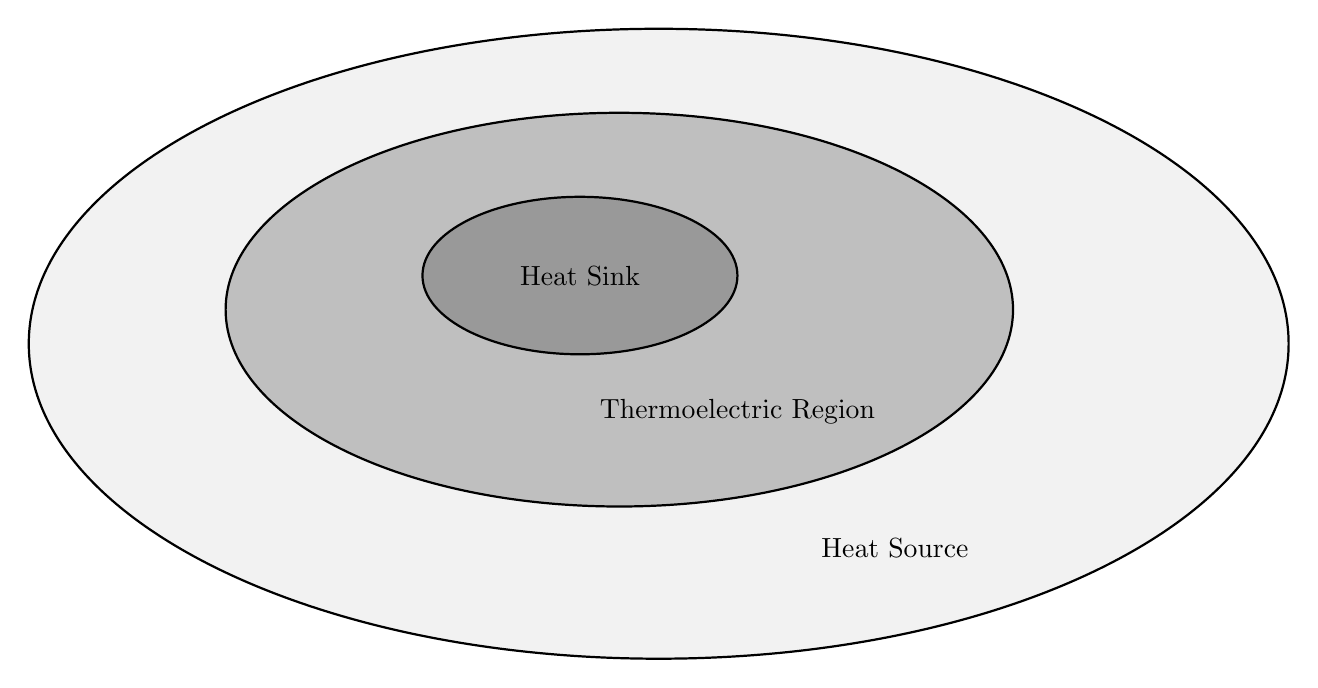
\begin{tikzpicture}
\def\angle{60}%
\pgfmathsetlengthmacro{\xoff}{2cm*cos(\angle)}%
\pgfmathsetlengthmacro{\yoff}{1cm*sin(\angle)}%
\draw [thick, fill=gray!10] (\xoff,-\yoff) circle[x radius=8cm, y radius=4cm] ++(3*\xoff,-3*\yoff) node{Heat Source};
\draw [thick, fill=gray!50] (0.5*\xoff,-0.5*\yoff) circle[x radius=5cm, y radius=2.5cm] ++(1.5*\xoff,-1.5*\yoff) node{Thermoelectric Region};
\draw [thick, fill=gray!80] (0,0) circle[x radius=2cm, y radius=1cm] node{Heat Sink};
\end{tikzpicture}

%ref for tikz: https://tex.stackexchange.com/questions/495446/drawing-concentric-ellipses-with-text-with-tikz

We modify the equations from [\ref{thermoelectric}], to radial equations.
Heat source and thermoelectric material in Fig.2[\ref{thermoelectric}] is now along the radius $r$. (\textcolor{red}{ASK ABOUT HARDWARE. Fig.1, and Fig.2. from ref})

Heat sink and resource for region $R$ are governed by the heat equation
\begin{equation}
\rho_R\ C_{vR}\ \frac{\partial T}{\partial t}=\nabla\cdot (k_R\nabla T),\label{heat}
\end{equation}

here, $T$ is the temperature, $t$ time, $\rho_R$ the density for region $R$, $C_{vR}$ specific heat, $k_R$ is the thermal conductivity. 

The middle layer is the thermoelectric region, governed by 
\begin{align}
\rho_{m}\ C_{vm}\ \frac{\partial T}{\partial t}&=\sigma\bE\cdot\bE-\sigma\cdot \alpha\bE\cdot \nabla T+\nabla\cdot[(k_m+\sigma\alpha^2T)\nabla T-\sigma\alpha T\bE],\label{elec}\\
\frac{\partial \rho}{\partial t}&=\nabla\cdot (-\sigma\bE+\sigma\alpha\nabla T).\label{chargedensity}
\end{align}
Here $\bE$ is the electric field, $\rho$ the charge density, $\sigma$ the electric conductivity, and $\alpha$ the Seebeck coefficient (\textcolor{red}{with temp dependence $\alpha=\alpha(T)$. Need curve fitting to decide}). 

\textcolor{red}{DO NOT KNOW ANY PARAMETERS}

\subsection{Reduction to 1D problem}
Based on our assumptions, we reduce spatial dependence to only on radius $r$: 
\begin{align}
\rho_R\ C_{vR}\ \frac{\partial T}{\partial t}&=\frac{\partial }{\partial r}\big(k_R\frac{\partial T}{\partial r}\big),\label{heat1d}\\
\rho_{m}\ C_{vm}\ \frac{\partial T}{\partial t}&=\sigma E^2-\sigma \alpha E\cdot \frac{\partial T}{\partial r}+\frac{\partial }{\partial r}[(k_m+\sigma\alpha^2T)\frac{\partial T}{\partial r}-\sigma\alpha T E],\label{elec1d}\\
\epsilon\frac{\partial E}{\partial t}&=J_0-\sigma E+\sigma\alpha\frac{\partial T}{\partial r}.\label{chargedensity1d}
\end{align}

Here \eqref{chargedensity1d} is the result of integrating \eqref{chargedensity}, and $J_0$ a constant. 

\subsection{Radial boundary conditions}

From outside inwards, the boundary conditions are:
\begin{itemize}
\item Outside: tree bark has $T_{amb}$.
\item Between Heat Source and Thermoelectric region, a voltage $V_0$ is generated, \textcolor{red}{heat flux and temperature??}
\item \textcolor{red}{section A. in Yan paper}

\end{itemize}

\newpage
Reference\textcolor{red}{BAD FORMAT. FOR convience only}
\begin{enumerate}
%%%%%%%%%%%% A
\item Time-Dependent Finite-Volume Model of Thermoelectric Devices, Yan. D. et al, IEEE, Transactions on industry applications, Vol. 50, No.1, Jan/Feb 2014\label{thermoelectric}

\item MIT notes online\label{mit}



\end{enumerate}




\end{document}
